%%%%%%%%%%%%%%%%%%%%%%%%%%%%%%%%%%%%%%
% Numerical Linear Algebra class 2022 
% Solutions to Sheet 3
%%%%%%%%%%%%%%%%%%%%%%%%%%%%%%%%%%%%%%

\begin{SolutionSheet}[\ref{sheet3}]
  \begin{onehalfspace}
    

  \begin{Solution} $A \in \C^{n\x n}$ hermitian, $ \ Q: \C^m \to \C^n \ (m<n) \ $ unitary, linear \\
    $B = Q^*AQ \in \C^{m \x m}$ \\
    \\
    \Claim $\forall\lambda_k \in\sigma(B): \quad \lambda_k =0$ or \begin{equation*}
        |\lambda_{min}(A)| \leq |\lambda_k (B)| \leq |\lambda_{max}(A)|
      \end{equation*}
    \Proof Let $v\in \C^m, v\neq 0.$ \\
    \\
    $\begin{array}{lll}
     \implies & \lambda_{max}(B) &\stackrel{\textit{Courant Fischer}}{=} \ \max_{v\in \C^m} \frac{v^*Bv}{v^*v} \\
      &&= \max_{v\in \C^m} \frac{v^*Q^*AQv}{v^*v} \\
      &&= \max_{w \in range(Q)} \frac{w^*Aw}{w^*(Q^*)^{-1}Q^{-1}w} \\
      && \leq \max_{w\in \C^n} \frac{w^*Aw}{w^*w} \\
      &&\stackrel{\textit{Courant Fischer}}{=} \lambda_{max}(A)
    \end{array}\\
    \\
    \implies |\lambda_k(B)| \leq |\lambda_{max}(A)| \quad \forall k = 1,...,n$\\
    (Other estimate analogous to max.)
  \end{Solution}

  \begin{Solution}
    $A$ diagonizable, real \\
    $\sigma(A) = \{-2, \ 1-2i, \ 1+2i, \ 1, \ -i, \ i, \ 2\}$ \\
    The power method converges to $\lambda\in \sigma(A)$ such that \begin{equation*}
      |\lambda - \sigma| = max
    \end{equation*} 
    $\implies $ does not converge for \begin{equation*}
      max = |\lambda_i -\sigma| = |\lambda_j - \sigma| \qquad (\lambda_i \neq \lambda_j)
    \end{equation*} 
    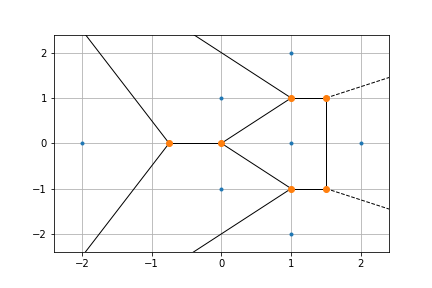
\includegraphics[width=7cm]{include/sheet3_ex2.png}\\
    (b) Wikipedia: \begin{equation*}
      \text{error} = \mathcal{O}\big(\frac{|\mu -\lambda_1|}{|\mu -\lambda_2|}\big) 
    \end{equation*}
    where $\lambda_1$ is the eigenvalue closest to $\sigma$, $\lambda_2$ the second closest.\\
    \\
    To find $\lambda = 2$:\\
    $\begin{array}{ll}
      \sigma > 2 &\implies \frac{1}{10} \geq \frac{\sigma - 2}{\sigma - 1}\\
        &\iff \frac{1}{10}\sigma - \frac{1}{10} \geq \sigma - 2 \\
        &\iff 2-\frac{1}{10} \geq \frac{9}{10}\sigma \\
        &\iff \frac{19}{9} \geq \sigma \\
        \\
      1 < \sigma < 2 &\implies \frac{1}{10} \geq \frac{2-\sigma}{\sigma -1} \\
       &\iff \frac{1}{10}\sigma - \frac{1}{10} \geq 2-\sigma \\
       &\iff \frac{11}{10}\sigma \geq \frac{21}{10} \\
       &\iff \sigma \geq \frac{21}{10}
    \end{array}\\
    \implies \text{ for }  \lambda=2  \text{ choose shift } \sigma\in  [\frac{21}{11}, \frac{19}{9}] $
  \end{Solution}

  \begin{Solution} Find shift parameters for $A= \begin{pmatrix}
    100 & 15 & 3 \\
    15 & 20 & 5 \\
    3 & 5 & 65
  \end{pmatrix}$\\
  Use Gershgorin Circle Theorem to obtain the circles: \\
  $D_1(100,18), \ D_2(20,20), \ D_3(65,8) \quad$ \\
  i.e. the intervals: $I_1[92,118], \ I_2[0,40], \ I_3[57,73]$\\
  The intervals are distinct $ \ \implies \ $ there is exactly one eigenvalue in each interval \\
  $\implies$ choose centers of intervals as shifts 
  \end{Solution}

  \begin{Solution}[Programming]
  \end{Solution}

\end{onehalfspace}

\end{SolutionSheet}


%%% Local Variables: 
%%% mode: latex
%%% TeX-master: "main"
%%% End: 
